\documentclass{beamer}
\usepackage[orientation=portrait,size =ISESISEE, scale=2,debug]{beamerposter}
\mode<presentation>{\usetheme{MPI}}
\usepackage{chemformula}
\usepackage[utf8]{inputenc}
\usepackage[german, english]{babel} % required for rendering German special characters
\usepackage{siunitx} %pretty measurement unit rendering
\usepackage{hyperref} %enable hyperlink for urls
\usepackage{ragged2e}
\usepackage[font=scriptsize,justification=justified]{caption}
\usepackage{array,booktabs,tabularx}
\usepackage{comment}

\usepackage{helvet}
\renewcommand{\familydefault}{\sfdefault}


\includeonlyframes{onlyone}


\newcolumntype{Z}{>{\centering\arraybackslash}X} % centered tabularx columns
%\sisetup{per=frac,fraction=sfrac}

%%%%%%%%%%%%%%%%%%%%%%%%%%%%%%%%%%%%%%%%%%%%%%%%%%%%%%%%%%%%%%%%%%%%%%%%%%%%%%%
%%%%%%%%%%%%%%%%%%%%%%%%%%%%%%%%%%%%%%%%%%%%%%%%%%%%%%%%%%%%%%%%%%%%%%%%%%%%%%%
%%%%%%%%%%%%%%%%%%%%%%%%%%%%%%%%%%%%%%%%%%%%%%%%%%%%%%%%%%%%%%%%%%%%%%%%%%%%%%%

\title{\Large From Data to Dissemination: Creating Dashboards for Buffalo African-American Community-based Participatory Air Monitoring}
\author[Yong-Hun Suh, Eun-Hye Yoo]{%
  Yong-Hun Suh$^{1}$ \and Eun-Hye Yoo$^{2}$
}

\institute[1,2]{%
  $^{1}$Max Planck Institute for Security and Privacy, Data Science for Humanity Group, Bochum, Germany\\
  $^{2}$University at Buffalo, SUNY, Geography, Buffalo, New York, United States of America
}


\date{23-24 of November, 2022}

%%%%%%%%%%%%%%%%%%%%%%%%%%%%%%%%%%%%%%%%%%%%%%%%%%%%%%%%%%%%%%%%%%%%%%%%%%%%%%%
%%%%%%%%%%%%%%%%%%%%%%%%%%%%%%%%%%%%%%%%%%%%%%%%%%%%%%%%%%%%%%%%%%%%%%%%%%%%%%%
%%%%%%%%%%%%%%%%%%%%%%%%%%%%%%%%%%%%%%%%%%%%%%%%%%%%%%%%%%%%%%%%%%%%%%%%%%%%%%%

\begin{document}


\begin{frame}[label=onlyone]
%\vspace{1em}
%%%%%%%%%%%%%%%%%%%%%%%%%%%%%%%%%%%%%%%%%%%%%%%%%%%%%%%%%%%%%%%%%%%%%%%%%%%%%%%
%
%
%

\centering
\begin{minipage}[t]{.985\textwidth}

\begin{columns}[t]

\begin{column}{.967\textwidth}

\begin{myblock2c}{1. From Numbers to Information}
\vspace{-2.em}
\begin{columns}[t]
% The African-American community on the east side of Buffalo, New York, experiences a disproportionate burden of chronic disease compared to neighboring regions.

%Fine particulate matter ($\text{PM}_{2.5}$) poses significant health threats, and its concentrations can fluctuate dramatically across both space and time in urban conditions. In Buffalo, a single EPA sensor covers the entire metropolitan area, making the spatio-temporal variability of the pollution patterns obscured and leaving vulnerable communities uninformed. To address this data gap, we deployed a network of affordable PurpleAir sensors throughout the East Side of the city, generating high-resolution $\text{PM}_{2.5}$ measurements. However, complex data formats and limited accessibility prevented residents from leveraging this information. In response, we partnered with community members to co-design an interactive dashboard that visualizes spatio-temporal $\text{PM}_{2.5}$ variability in real time, empowering disadvantaged neighborhoods with actionable air quality insights.
\begin{column}{.54\textwidth}
\begin{justify}
Fine particulate matter ($\text{PM}_{2.5}$) poses significant health threats, and its spatial and temporal variability can be substantial. On the East Side of Buffalo, New York, the predominantly African-American residents face a disproportionate burden of chronic disease, which may be worsened by poor air quality. In the absence of localized monitoring, however, neighborhood-level pollution exposures have remained largely ignored. A small number of EPA sensors serves the entire Buffalo-Niagara metropolitan area, obscuring the spatio-temporal variability of air pollution and preventing vulnerable community members access to accurate air quality information. 
% \newline

To address this gap in data and equity, we partnered with local community members using community-based participatory research (CBPR) methods. We deployed a network of low-cost PurpleAir(PA) sensors across the East Side, generating high-resolution $\text{PM}_{2.5}$ data. Recognizing that raw data alone is insufficient, we co-designed an interactive dashboard with community members to visualize pollution patterns in real time, making air quality insights accessible, understandable, and relevant to those most affected.
\end{justify}

\vspace{1em}

\end{column}

\begin{column}{.01\textwidth}
\end{column}

\begin{column}{.45\textwidth}
% Dashboard figure
\vspace{-1em}
\begin{figure}[h]
\caption{Breathe Buffalo: UB Air Quality Monitoring Dashboard}
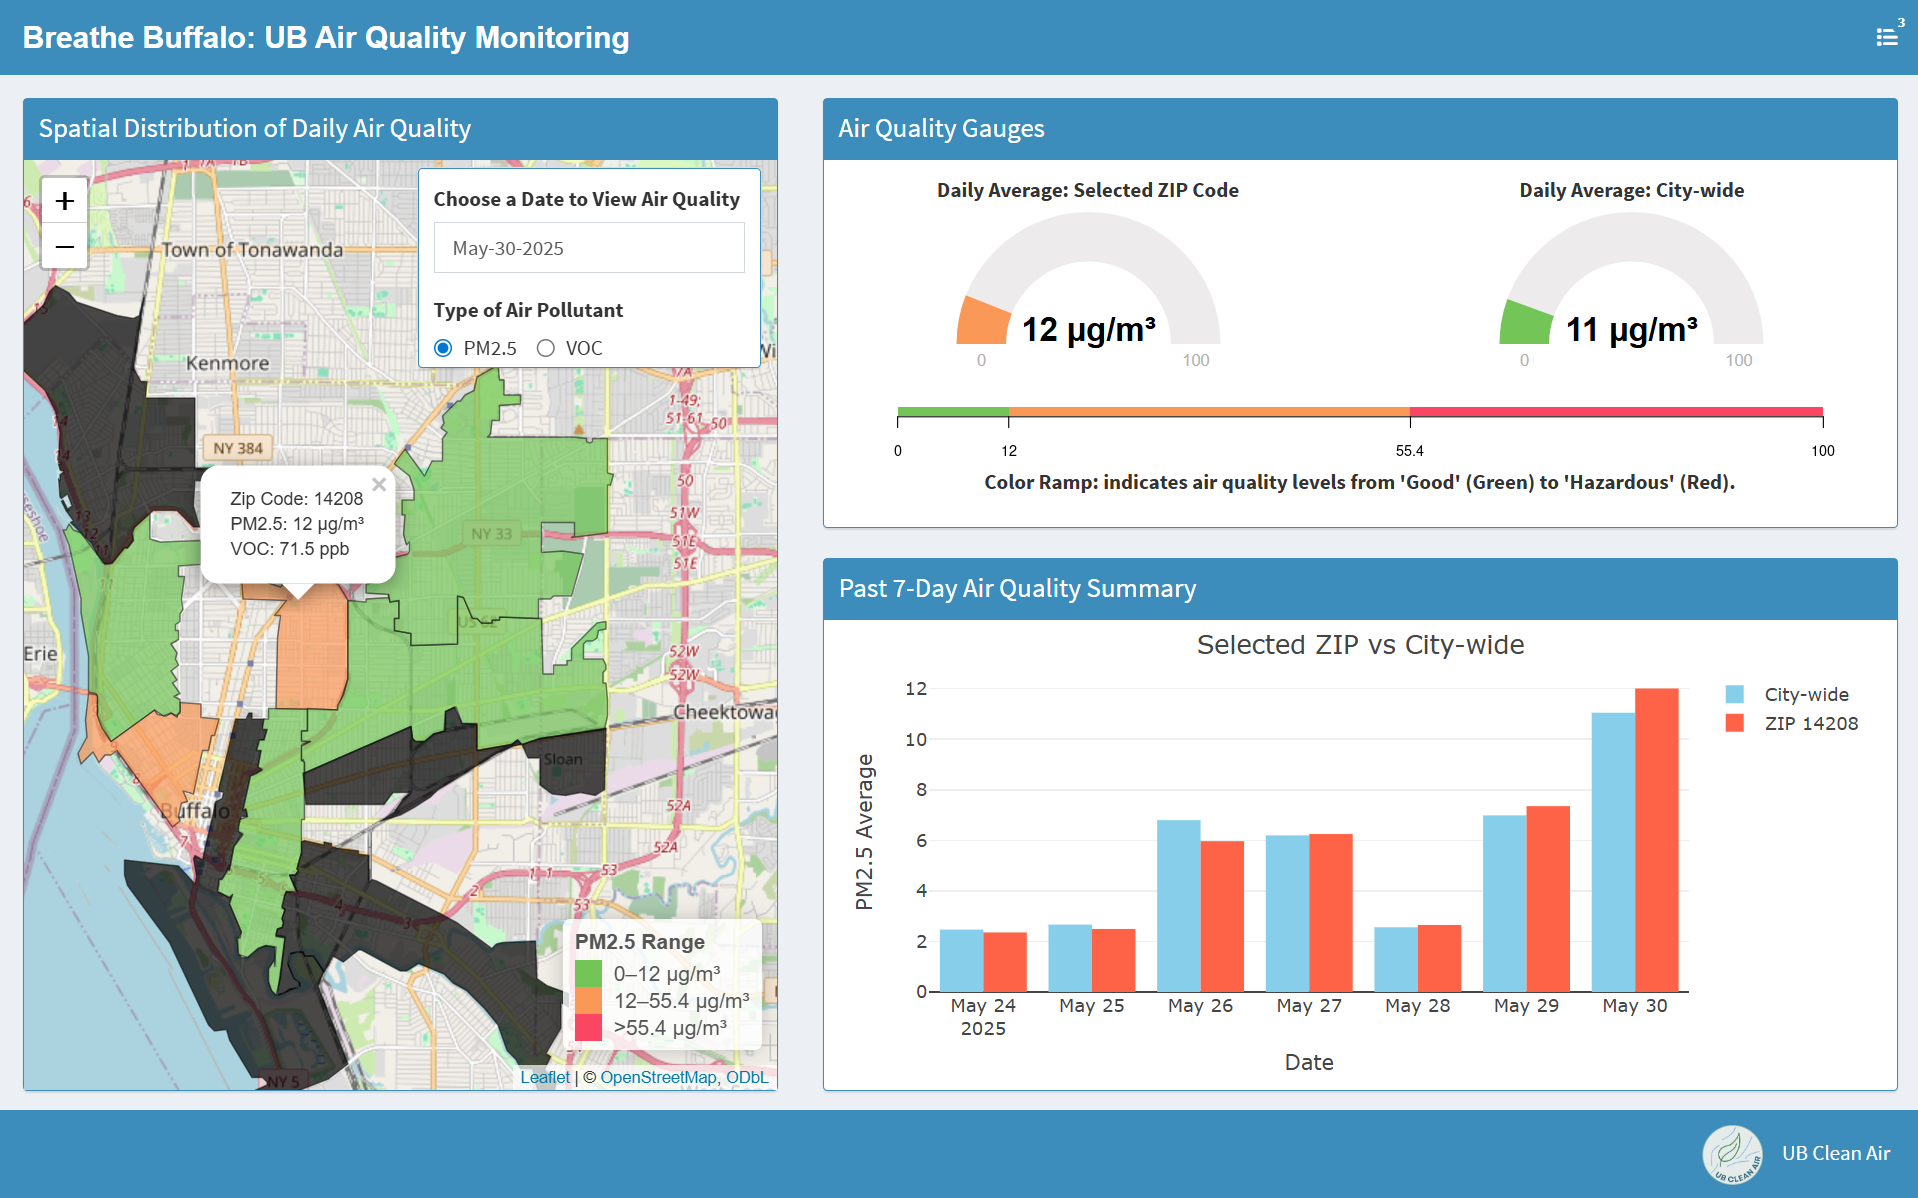
\includegraphics[width=\textwidth, keepaspectratio]{diagrams/Dashboard.png}
\end{figure}
\vspace{1em}


\end{column}

\end{columns}

\vspace{-.5em}

\end{myblock2c}


\end{column}

\end{columns}

\vspace{-1.1em}

\begin{columns}[t]
% Begin of the first column
\begin{column}{.47\textwidth}


\begin{myblock1c}{2. Objectives}
\vspace{-1em}

To design an effective interface for spatio-temporal variability of air quality for disadvantaged community members
\vspace{.3em}
  \begin{itemize}
  \item Co-design with community members to accommodate their mental models and priority needs for visualizing spatio-temporal air quality patterns
  \item Develop an interactive dashboard prototype that reflects those priorities and is easy to navigate

  \end{itemize}


\end{myblock1c}

%\begin{myblock2c}{Key Features - \url{https://eprint.iacr.org/2022/1270.pdf}}
\begin{myblock1c}{3. Methods}

\vspace{-2em}
\begin{columns}[t]
\begin{column}{.47\textwidth}

\textbf{\color{MPI2}Data Collection Strategy}
\begin{itemize} 
  \item Deployed 30 PA sensors in the study area
  \item Built a fully automated data collection pipeline
  \item Stored the data in a hosted Database, which can be retrieved by quires at anytime
\end{itemize}

\textbf{\color{MPI2}Dashboard}
\begin{itemize}
  \item Refined the interface through community-led sessions to capture what users need
  \item Incorporated accessible design with users in mind
  \item Used GitHub, ensuring easy deployment and reproducibility 
\end{itemize}

\end{column}

\begin{column}{.47\textwidth}
\begin{figure}[h]
\caption{Architecture Overview}
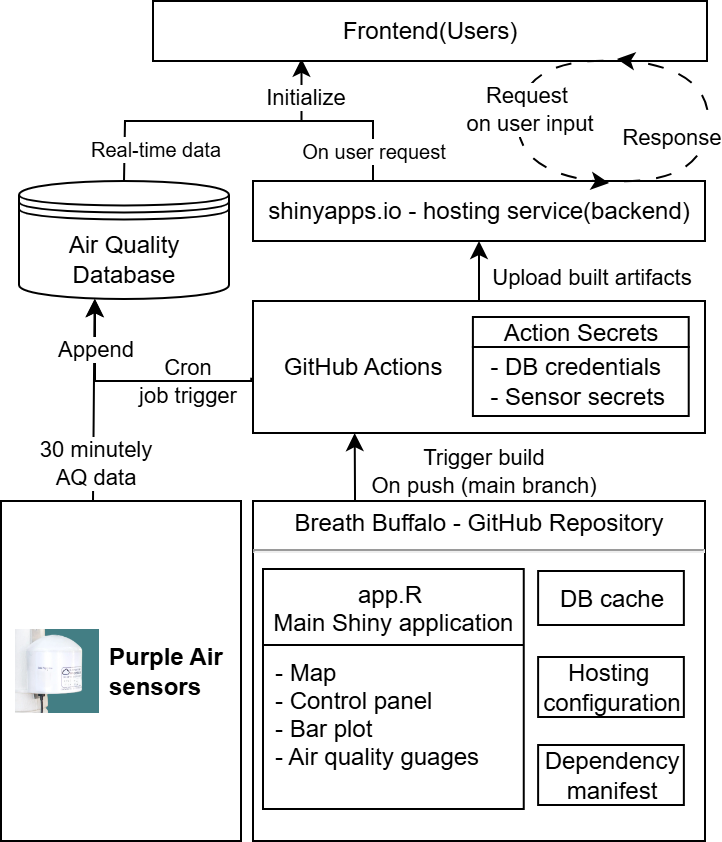
\includegraphics[width=\textwidth,   height=18cm,  keepaspectratio]{diagrams/BB_diagram.drawio_DB.png} %https://app.diagrams.net/
\end{figure}

\end{column}
\end{columns}

% We co-designed an online dashboard with our study participants to prototype PM and VOC reporting tools, using virtual meetings and surveys. This collaborative process resulted in a community-tailored platform that summarizes air monitoring and study design, featuring accessible color schemes, large fonts for key results, and interactive maps and plots. We implemented a CI/CD pipeline with GitHub Actions to ensure full reproducibility and automate testing and deployment of dashboard updates.

\begin{columns}[t]
\begin{column}{.47\textwidth}

\begin{figure}[h]
\caption{PurpleAir Sensor}
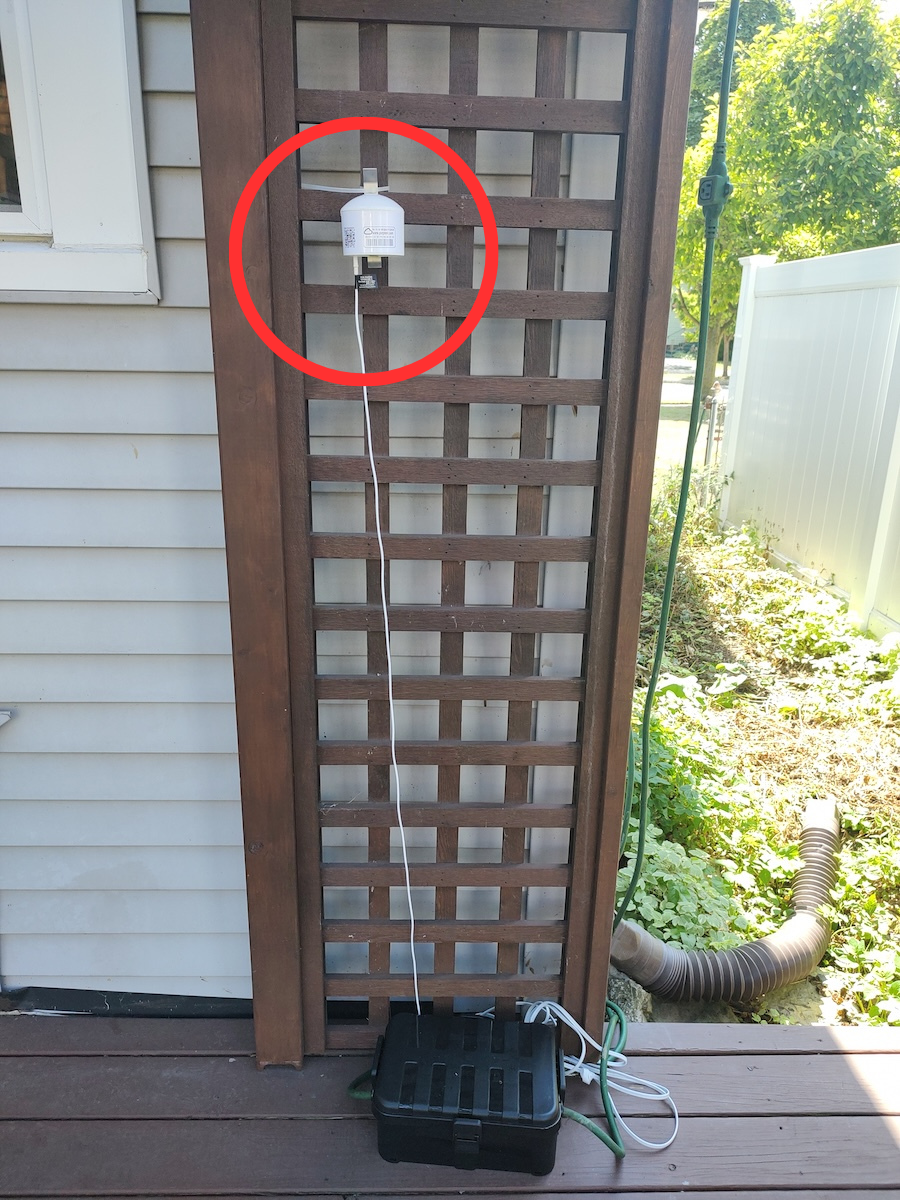
\includegraphics[width=\textwidth,  keepaspectratio]{diagrams/PA_highlighted.png}
\end{figure}

\vspace{1.2em}

\end{column}

\begin{column}{.47\textwidth}

\begin{figure}[h]
\caption{Calibrating PA Sensors}
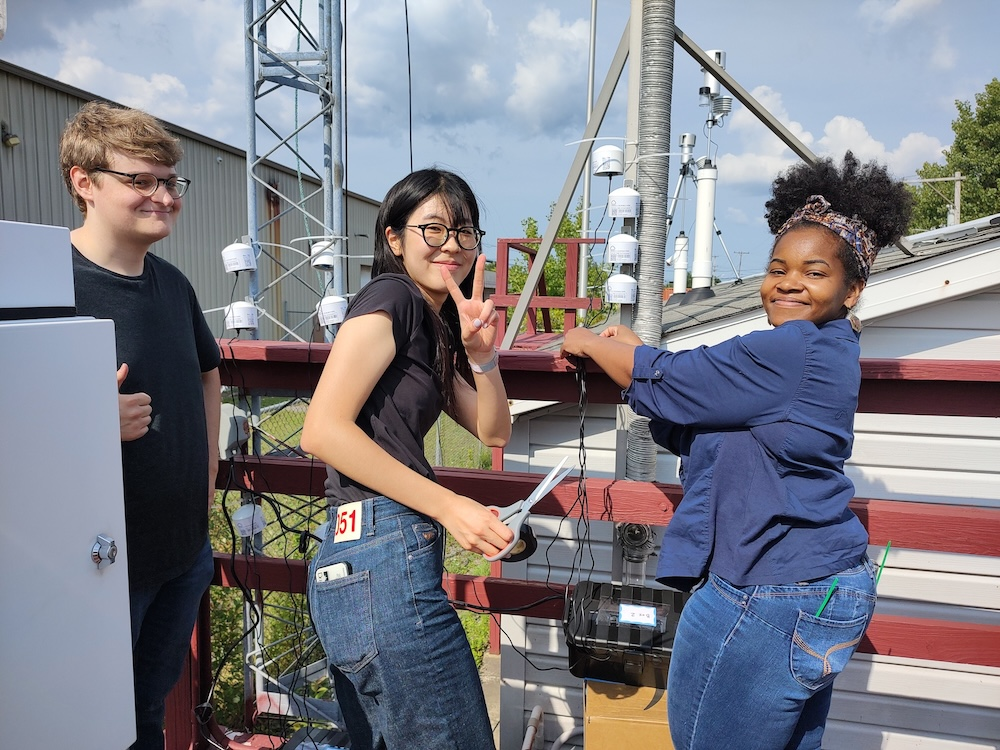
\includegraphics[width=\textwidth,  keepaspectratio]{diagrams/calibraiton_sites.jpg} 
\end{figure}

\end{column}
\end{columns}

\end{myblock1c}

\end{column}




\begin{column}{.47\textwidth}

\vspace{-.5em}
\begin{myblock1c}{4. Results}
\begin{flushleft}

\vspace{-1em}
\textbf{\color{MPI2}Visualizing Air Quality}
  \begin{itemize}
  \item \textbf{Visualization of Localized and Dynamic Variability of PM$_{2.5}$}:  \newline
  Shows the daily and community specific air quality using a map and graphics 
  \item \textbf{Comparison With The Baseline}:  \newline
  Provides both the community-specific air quality information and the city-wide air quality from EPA monitoring sites
  \end{itemize}

\textbf{\color{MPI2}User-friendly Dashboard}
  \begin{itemize}
  \item \textbf{Color-coded Components}: \newline
  Displays air quality data using a user-friendly color scheme in a map, a bar plot, and gauges with a reference color ramp
  \item \textbf{Interactive Dash}: \newline
  An interactive map with pop-up information and the controller for selecting the time and location
  \end{itemize}
\vspace{.2em}

\end{flushleft}

\end{myblock1c}

\begin{myblock1c}{5. Discussion}
\vspace{-1em}
\begin{itemize}
\item Co-developed a community-informed dashboard for real-time, accessible air quality data.
\item Empowered residents by providing localized and dynamic information on air pollution.
\item Future works can be expanded by using AI: \newline
- AI voiceover with multi-language support \newline
- Estimate air quality in areas without measurements using machine learning algorithms
\end{itemize}



\end{myblock1c}


\begin{myblock1c}{References}
\vspace{-1em}
\begin{flushleft}
\begin{itemize}
  \scriptsize\color{gray}
  \item Southerland, V. A., Brauer, M., Mohegh, A., Hammer, M. S., Van Donkelaar, A., Martin, R. V., ... \& Anenberg, S. C. (2022). Global urban temporal trends in fine particulate matter (PM2.5) and attributable health burdens: estimates from global datasets. \textit{The Lancet Planetary Health, 6}(2), e139–e146.

  \item Yan, D., Ji, H., Fu, H., Jiang, J., Su, B., \& Ye, B. (2024). The effect of fine particulate matter (PM2.5) pollution on health inequality: an intergenerational perspective. \textit{Environmental Geochemistry and Health, 46}(6), 195.
\end{itemize}
\end{flushleft}


\end{myblock1c}

\begin{myblock1c}{Give it a try yourself!}
\begin{flushleft}

\vspace{-2.5em}

\end{flushleft}
\begin{columns}

\begin{column}{.5\textwidth}
\begin{figure}[h]
\caption*{Breath Buffalo}

\includegraphics[width=7cm, keepaspectratio]{diagrams/BB_QR.png}
\end{figure}

\end{column}


\begin{column}{.5\textwidth}

\begin{figure}[h]
\caption*{Source Code (GitHub)}

\includegraphics[width=7cm, keepaspectratio]{diagrams/QR-for-YONGHUNI.png}
\end{figure}

\end{column}
\end{columns}


\end{myblock1c}

\end{column}
\end{columns}




% \begin{columns}

% \begin{column}{.965\textwidth}

% \begin{myblock1c}{Conclusions \& Future Directions}


% \end{myblock1c}
% \end{column}


% %
% %


% \end{columns}



\end{minipage}

%
%
%
%%%%%%%%%%%%%%%%%%%%%%%%%%%%%%%%%%%%%%%%%%%%%%%%%%%%%%%%%%%%%%%%%%%%%%%%%%%%%%%


\end{frame}
\end{document}
